\documentclass[aspectratio=169, 14pt]{beamer}
\usepackage[utf8]{inputenc}
\usepackage[english]{babel}
\usepackage{tipa}
\usepackage{graphicx}
\usepackage{transparent}
\usepackage[ruled, lined, linesnumbered, commentsnumbered]{algorithm2e}
\usepackage{tikz}
\usetikzlibrary{calc,shadows.blur}
\usetikzlibrary{matrix,backgrounds}
\usetikzlibrary{arrows, positioning}
\usetikzlibrary {arrows.meta}
\usetikzlibrary{decorations.pathmorphing, patterns}
\pgfdeclaredecoration{penciline}{initial}{
    \state{initial}[width=+\pgfdecoratedinputsegmentremainingdistance,auto corner on length=1mm,]{
        \pgfpathcurveto%
        {% From
            \pgfqpoint{\pgfdecoratedinputsegmentremainingdistance}
                            {\pgfdecorationsegmentamplitude}
        }
        {%  Control 1
        \pgfmathrand
        \pgfpointadd{\pgfqpoint{\pgfdecoratedinputsegmentremainingdistance}{0pt}}
                        {\pgfqpoint{-\pgfdecorationsegmentaspect\pgfdecoratedinputsegmentremainingdistance}%
                                        {\pgfmathresult\pgfdecorationsegmentamplitude}
                        }
        }
        {%TO 
        \pgfpointadd{\pgfpointdecoratedinputsegmentlast}{\pgfpoint{1pt}{1pt}}
        }
    }
    \state{final}{}
}
\usepackage{minted}
\usepackage{csquotes}
\usepackage{outlines}
\usepackage{booktabs}
\usepackage{hyperref}
\hypersetup{
    colorlinks=true,
    linkcolor=blue,
    filecolor=magenta,      
    urlcolor=cyan,
    }
\urlstyle{same}
\usetheme{metropolis}
\metroset{block=fill}
\usecolortheme{default}
\definecolor{darkmidnightblue}{rgb}{0.0, 0.2, 0.4}
\definecolor{LightGray}{gray}{0.9}


%------------------------------------------------------------
%This block of code defines the information to appear in the
%Title page
\title[Data Structures] %optional
{Data Structures}

\subtitle{Stacks}

\author[CHEN Zhongpu] % (optional)
{CHEN Zhongpu}

\institute[] % (optional)
{
  School of Computing and Artificial Intelligence \\
  \href{mailto:zpchen@swufe.edu.cn}{zpchen@swufe.edu.cn}
}

\date[] % (optional)
{SWUFE, Fall 2022}

%End of title page configuration block
%------------------------------------------------------------


%------------------------------------------------------------
%The next block of commands puts the table of contents at the 
%beginning of each section and highlights the current section:

% \AtBeginSection[]
% {
%   \begin{frame}
%     \frametitle{Table of Contents}
%     \tableofcontents[currentsection]
%   \end{frame}
% }
%------------------------------------------------------------


\begin{document}

%The next statement creates the title page.
\frame{\titlepage}

%---------------------------------------------------------
%This block of code is for the table of contents after
%the title page
% \begin{frame}
% \frametitle{Table of Contents}
% \tableofcontents
% \end{frame}
%--------------------------------------------------------
\begin{frame}[fragile]
    \frametitle{A Small Quiz}
    \begin{enumerate}
        \item Someone claims that ``the complexity of this algorithm is $O(n\log{n})$''. What does she mean?
        \item What is time complexity of the following code?
    \end{enumerate}

\begin{minted}[bgcolor=LightGray]{java}
double m = a[0];
for (int i = 1; i < N; i++)
    if (a[i] > m) m = a[i];
\end{minted}  

\end{frame}

\begin{frame}[fragile]
    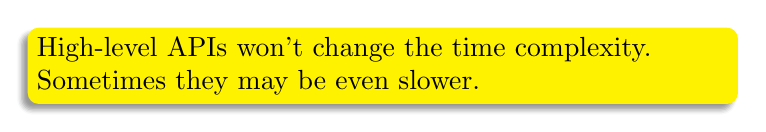
\begin{tikzpicture}
        \node[fill=yellow,blur shadow={shadow xshift=-0.5ex},
        text width=25em,anchor=south west,rounded corners]
        {High-level APIs won't change the time complexity. Sometimes they may be even slower.
        };
    \end{tikzpicture} 
    \begin{minted}[bgcolor=LightGray]{java}
double[] a = {3.14, 2.7, 9.8, 6.7, 8};
double m = Arrays.stream(a).max().getAsDouble();
    \end{minted}  

\begin{minted}[bgcolor=LightGray]{python}
a = [3.14, 2.7, 9.8, 6.7, 8]
m = max(a)
\end{minted} 

\end{frame}

{
    % \usebackgroundtemplate{\transparent{0.3}{\begin{picture}
    %     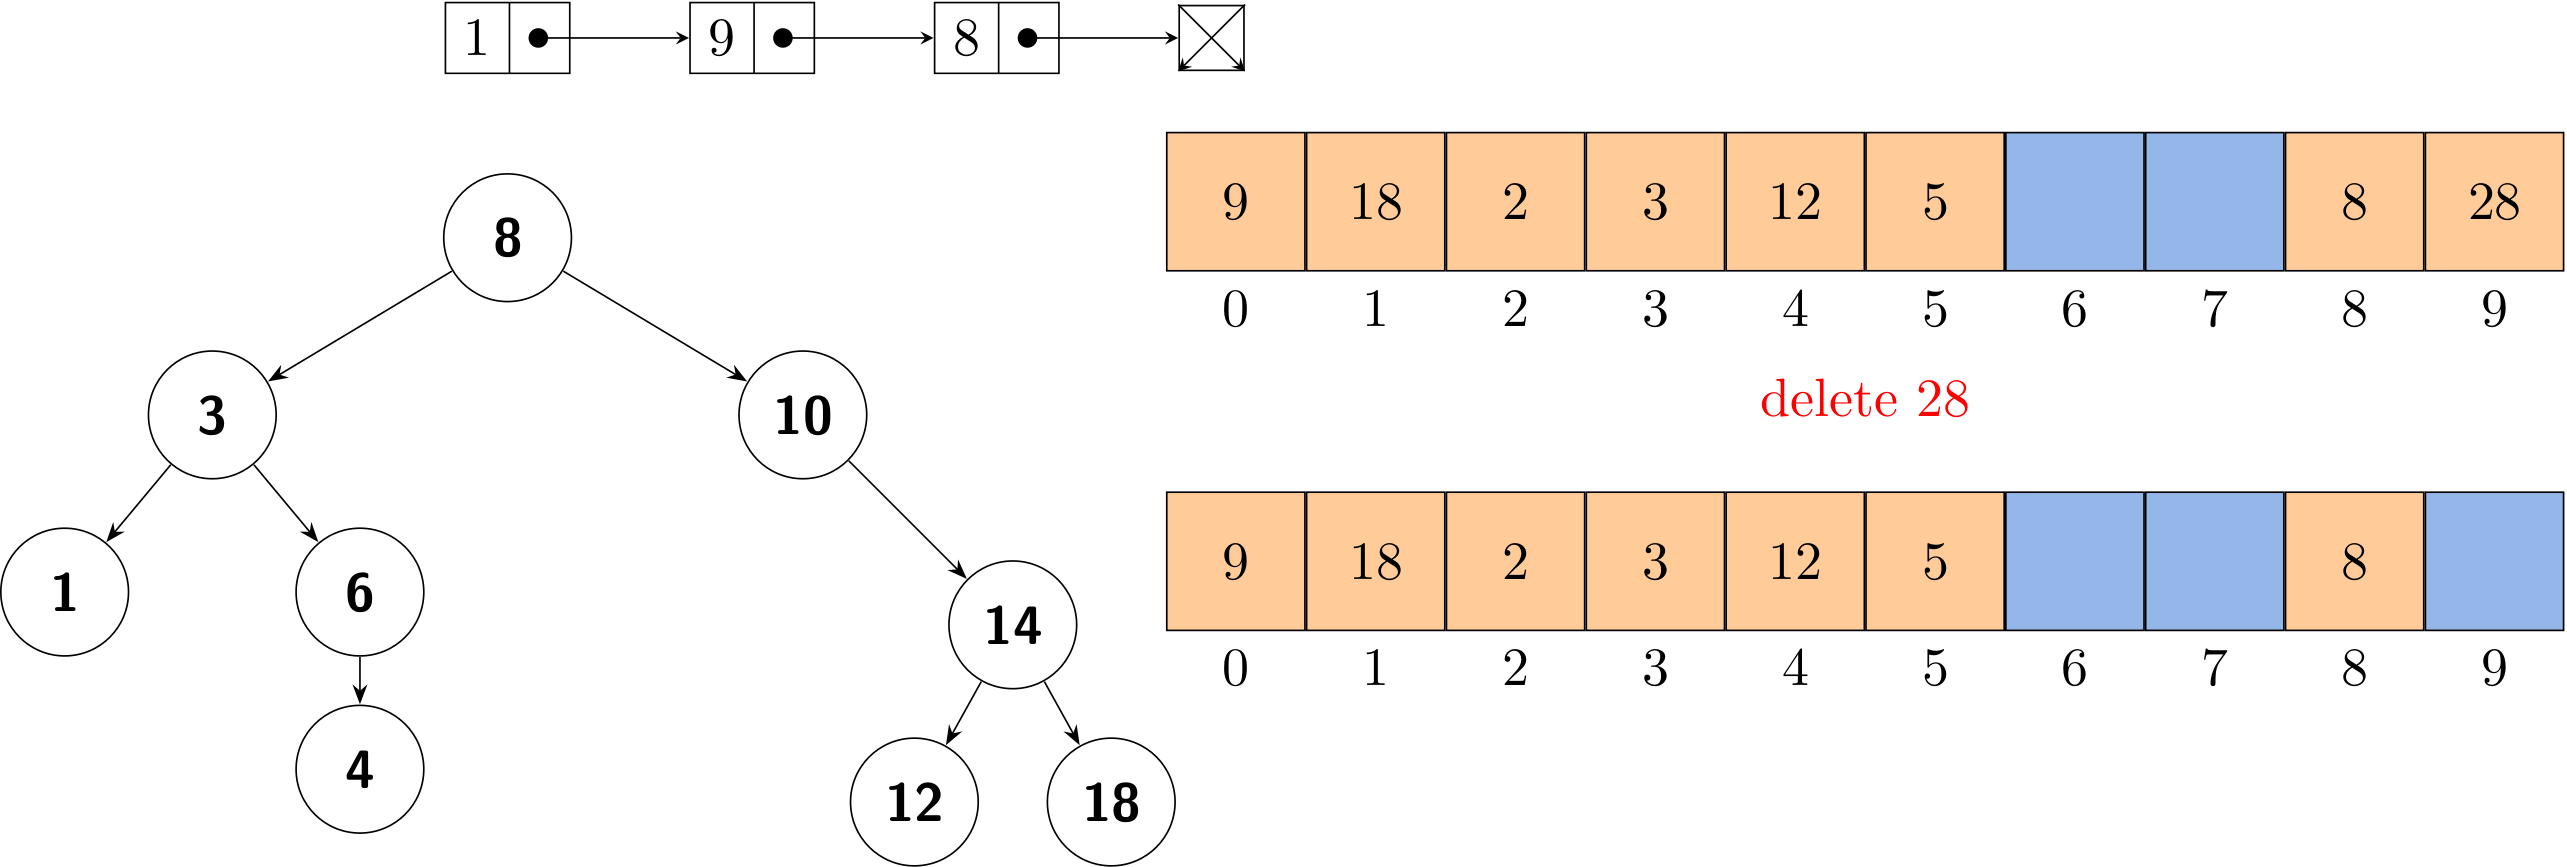
\includegraphics[height=0.7\paperheight]{cover}
    % \end{picture}    
    % }}
\usebackgroundtemplate{
  \tikz[overlay,remember picture] 
  \node[opacity=0.3, at=(current page.south east),anchor=south east, yshift=2cm,xshift=4cm] {
    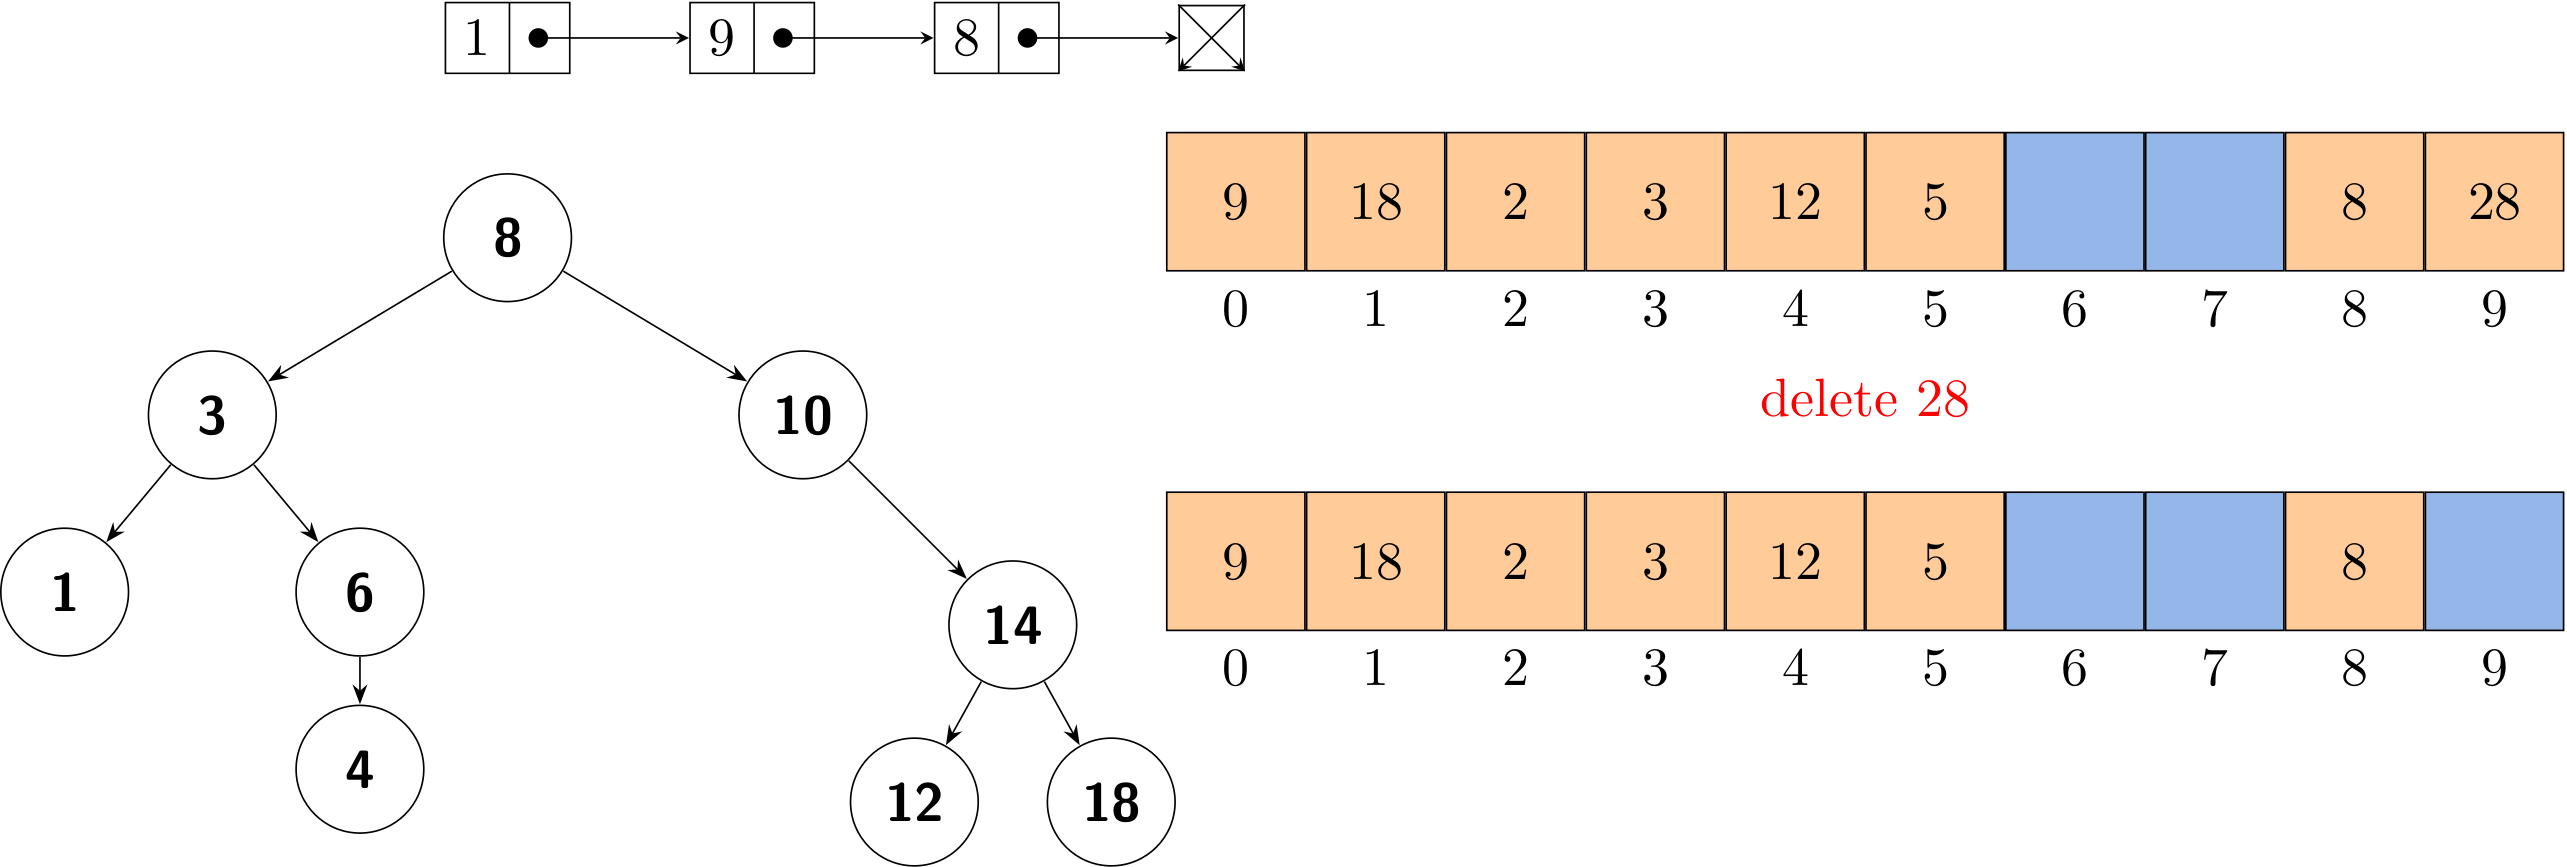
\includegraphics[height=0.6\paperheight]{cover}};
}
    \begin{frame}
        \section{\textcolor{darkmidnightblue}{Stacks}}
    \end{frame}
}

\begin{frame}[fragile]
    \frametitle{Web Pages}

    \begin{columns}
        \column{0.5\textwidth}
        \begin{verbatim}
<!-- a.html -->
<a href="b.html">Next</a>

<!-- b.html -->
<a href="c.html">Next</a>

<!-- c.html -->
<a href="d.html">Next</a>
        \end{verbatim}
        \column{0.5\textwidth} 
        Suppose you are visiting \textbf{a.html}, and then click ``Next''. Continue to click ``Next'' until reaching \textbf{d.html}. Now start to consider click ``Back''.
    \end{columns}

\end{frame}

\begin{frame}
    \begin{quote}
        Stack: a pile of things arranged one on top of another.
        \begin{flushright}
            --- from Cambridge dictionary
        \end{flushright}
    \end{quote}
    \pause
    \begin{figure}
        
\includegraphics[width=0.4\textwidth, height=0.4\paperheight]{week3/book}
        \hfill
        
\includegraphics[width=0.4\textwidth, height=0.4\paperheight]{week3/tray}
    \end{figure}
    \pause
    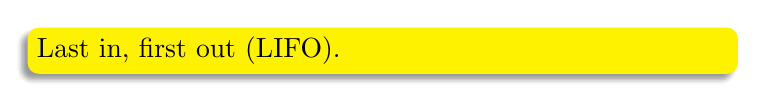
\begin{tikzpicture}
        \node[fill=yellow,blur shadow={shadow xshift=-0.5ex},
        text width=25em,anchor=south west,rounded corners]
        {Last in, first out (LIFO).
        };
    \end{tikzpicture} 
\end{frame}

\begin{frame}
    \frametitle{Stack}
\begin{exampleblock}{Stack}
    A stack is a collection of objects that are inserted and removed according to the \alert{last-in, first-out (LIFO)} policy. 
\end{exampleblock}
It supports two basic operations:
\begin{itemize}
    \item \texttt{push()}: add a new element
    \item \texttt{pop()}: remove an element
\end{itemize}
Additionally, it also supports other operations such as \texttt{size()}, \texttt{isEmpty()}.
\end{frame}

\begin{frame}[fragile]
    \frametitle{Stack in Python}
    Fortunately, the \texttt{list} in Python supports the operations required by stacks.
\begin{minted}[bgcolor=LightGray]{python}
s = []
s.append('a') # append() works like push()
s.append('b')
s.append('c')
print(len(s))
print(s.pop())
print(s.pop())
print(len(s))
\end{minted}     

\end{frame}

\begin{frame}[fragile]
But, we would like a \alert{Stack} class which allows us to write code in the object-oriented way. 
\begin{minted}[bgcolor=LightGray]{python}
s = Stack()
s.push('a')
s.append('b')
s.append('c')
print(s.size())
print(s.pop())
print(s.pop())
print(s.size())
\end{minted}      

\end{frame}

\begin{frame}[fragile]

\begin{minted}[baselinestretch=0.9,bgcolor=LightGray]{python}
class Stack:
    def __init__(self):
        self._data = []

    def push(self, item):
        pass

    def pop(self):
        pass

    def size(self):
        pass

    def is_empty(self):
        pass
\end{minted}     

\end{frame}

\begin{frame}[fragile]
    \begin{minted}[bgcolor=LightGray]{python}
def push(self, item):
    self._data.append(item)    
\end{minted}

\begin{minted}[bgcolor=LightGray]{python}
def pop(self):
    return self._data.pop()   
\end{minted}

    \begin{minted}[bgcolor=LightGray]{python}
def size(self):
    return len(self._data)    
    \end{minted}
\pause
Another operation \texttt{top()} (a.k.a., \texttt{peek()}) is often used. It works like \texttt{pop()}, but it doesn't delete the element.
\end{frame}

\begin{frame}[fragile]
\begin{block}{Exception}
    You need also consider the condition that cannot be handley by the ``normal flow''.
\end{block}

What will happen if we \texttt{pop} from an empty stack?
\begin{minted}[bgcolor=LightGray]{python}
s = Stack()
print(s.pop())   
\end{minted}

\pause

\begin{minted}[baselinestretch=0.9,bgcolor=LightGray]{python}
def pop(self):
    if self.is_empty():
        raise NoElement('Pop from empty stack!')
    return self._data.pop()  
\end{minted}

\end{frame}

\begin{frame}
    \frametitle{Time complexity}
    \begin{table}
        \caption{Stack's time complexity}
        \begin{tabular}{lr}
          \toprule
          Operation & Complexity\\
          \midrule
          \texttt{push()} & $O(1)$\\
          \texttt{pop()} & $O(1)$ \\
          \texttt{size()} & $O(1)$ \\
          \texttt{is\_empty()} & $O(1)$ \\ 
          \bottomrule
        \end{tabular}
    \end{table}

    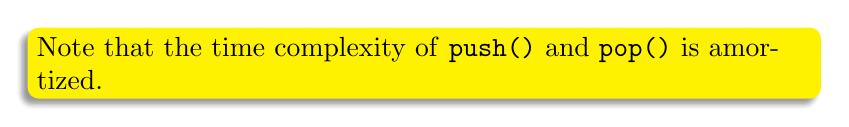
\begin{tikzpicture}
        \node[fill=yellow,blur shadow={shadow xshift=-0.5ex},
        text width=28em,anchor=south west,rounded corners]
        {Note that the time complexity of \texttt{push()} and \texttt{pop()} is amortized. 
        };
    \end{tikzpicture} 
\end{frame}

\begin{frame}[fragile]
    \frametitle{Resizing}
Basically, an amortized time is \textbf{the average time taken per operation, if you do many operations}.

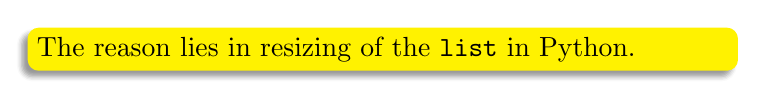
\begin{tikzpicture}
    \node[fill=yellow,blur shadow={shadow xshift=-0.5ex},
    text width=25em,anchor=south west,rounded corners]
    {The reason lies in \alert{resizing} of the \texttt{list} in Python. 
    };
\end{tikzpicture}
\pause
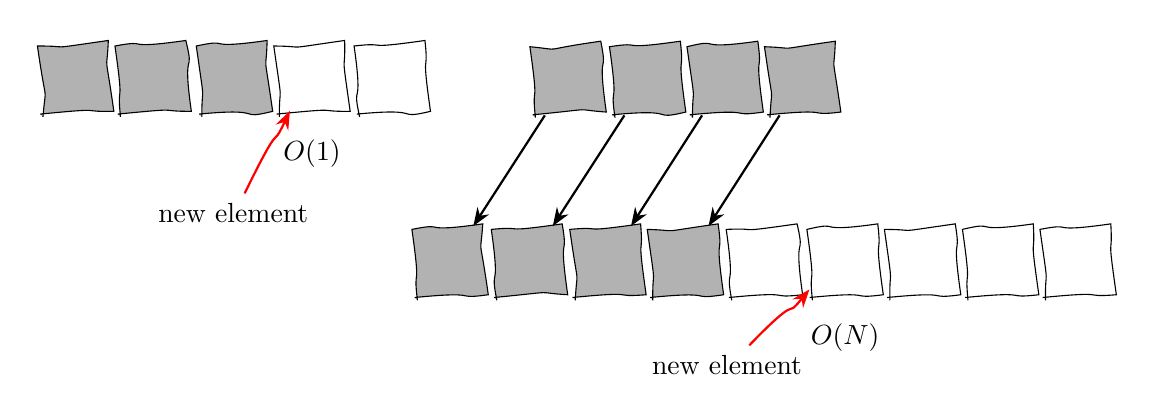
\begin{tikzpicture}[slot/.style={minimum size=0.9cm,rectangle}, data/.style={slot, fill=black!30}, >=Stealth, decoration=penciline]
\matrix [nodes=draw] (table1)
{
  \node[data, decorate] {}; &
  \node[data, decorate] {}; &
  \node[data, decorate] {}; & 
  \node[slot, decorate] (insert) {}; &
  \node[slot, decorate] {}; 
  \\ 
};
\node[below=of insert, xshift=-1cm] (start) {new element};
\draw[->,thick,red, decorate] (start) -- (insert);
\node[below=of insert, yshift=0.8cm] {$O(1)$};

\matrix [nodes=draw, right=of table1](table2)
{
  \node[data, decorate] (2n1) {}; &
  \node[data, decorate] (2n2) {}; &
  \node[data, decorate] (2n3) {}; & 
  \node[data, decorate] (2n4) {}; 
  \\ 
};

\matrix [nodes=draw, below=of table2, xshift=1cm](table3)
{
  \node[data, decorate] (3n1) {}; &
  \node[data, decorate] (3n2) {}; &
  \node[data, decorate] (3n3) {}; & 
  \node[data, decorate] (3n4) {}; &
  \node[slot, decorate] {}; &
  \node[slot, decorate] (insert2) {}; & 
  \node[slot, decorate] {}; & 
  \node[slot, decorate] {}; & 
  \node[slot, decorate] {};  
  \\ 
};

\draw[->, thick] (2n1) -- (3n1);
\draw[->, thick] (2n2) -- (3n2);
\draw[->, thick] (2n3) -- (3n3);
\draw[->, thick] (2n4) -- (3n4);

\node[below=of insert2, xshift=-1.5cm, yshift=0.4cm] (start2) {new element};
\draw[->,thick,red, decorate] (start2) -- (insert2);
\node[below=of insert2, yshift=0.8cm] {$O(N)$};

\end{tikzpicture}

\end{frame}

\begin{frame}[fragile]
Bob devises a new implementation for stacks based on the \texttt{list}. 

\begin{itemize}
    \item \texttt{push()}: insert the new element in the front of the \texttt{list}
    \item \texttt{pop()}: remove and return the first element of the \texttt{list}
\end{itemize}

\begin{minted}[baselinestretch=1,bgcolor=LightGray]{python}
s = []
s.insert(0, 'a')
s.insert(0, 'b')
s.insert(0, 'c')
print(s.pop(0)) # 'c'
print(s.pop(0)) # 'b'
\end{minted}  
    
How do you think of his idea?
\end{frame}

\begin{frame}

\begin{center}
    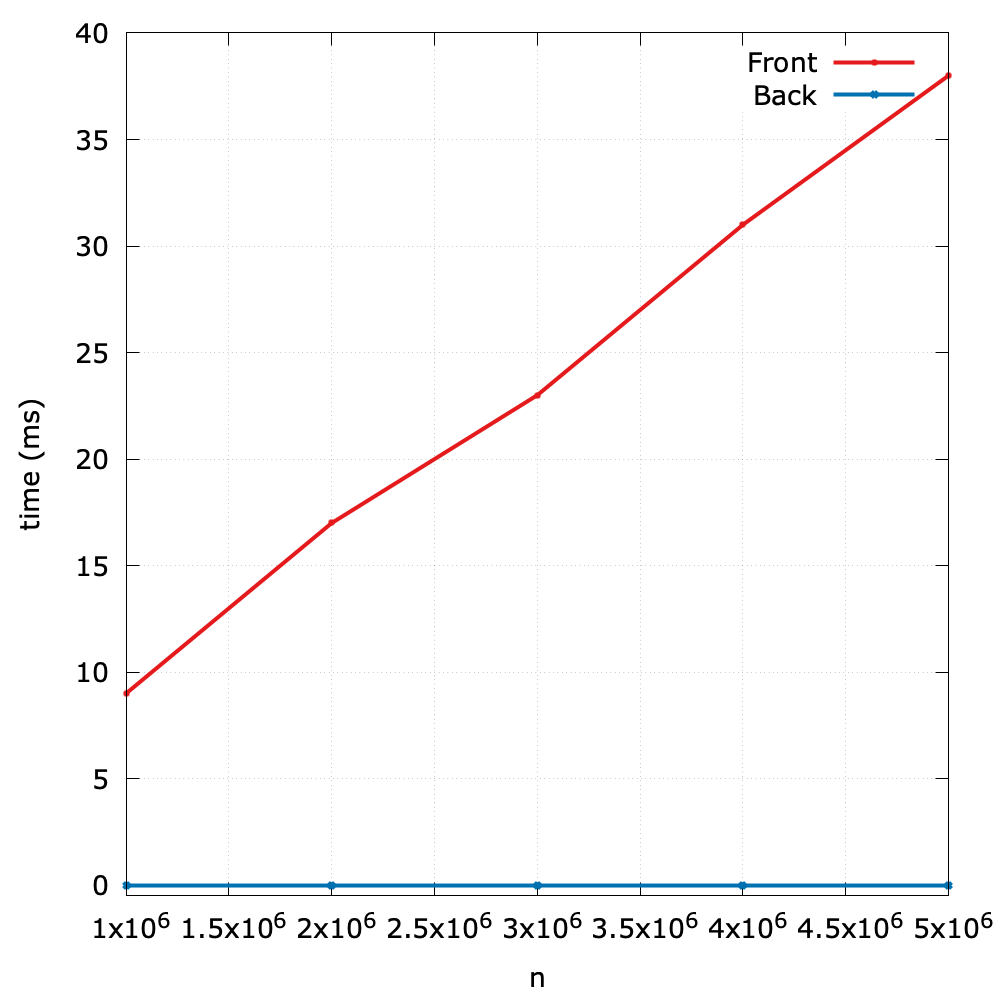
\includegraphics[height=.98\paperheight]{week3/front-back}
\end{center}    

\end{frame}

\begin{frame}
    \frametitle{Matching Parentheses}

    Here we assume that only parentheses $()$, braces $\{\}$, and brackets $[]$ are allowed.

    Clearly, each opening symbol must match its corresponding closing symbol. For example:

    \begin{itemize}
        \item Correct: $()(())\{([()])\}$
        \item Incorrect: $(\{[])\}$
    \end{itemize}

\end{frame}

\begin{frame}[fragile]
    \begin{minted}[baselinestretch=1.1,bgcolor=LightGray]{python}
def is_matched(expr):
    openings = '([{'
    closings = ')]}'
    s = Stack()
    for c in expr:
        if c in openings:
            s.push(c)
        elif c in closings:
            if s.is_empty():
                return False
            if TODO:
                return False
    return s.is_empty()
    \end{minted}  

\end{frame}

\begin{frame}[fragile]
    \frametitle{Iterator}
    The \alert{iterator} behind the scenes plays the magic:

    \begin{columns}
        \column{0.475\textwidth}
        \begin{minted}[bgcolor=LightGray]{python}
a = [1, 9, 4, 6]
for i in a:
    print(i)    
    \end{minted}
        \column{0.475\textwidth} 
        \begin{minted}[bgcolor=LightGray]{python}
s = Stack()
s.push(1)
s.push(2)
s.push(3)
for i in s:
    print(i)
    \end{minted}

    \end{columns}
\end{frame}

\begin{frame}[fragile]
    \begin{minted}[baselinestretch=1,bgcolor=LightGray]{python}
class ReverseListIterator:
    def __init__(self, data):
        self._data = data
        self._i = len(data)

    def __next__(self):
        if self._i == 0:
            raise StopIteration
        self._i -= 1
        return self._data[self._i]  
    \end{minted}

        \begin{minted}[bgcolor=LightGray]{python}
def __iter__(self):
    return ReverseListIterator(self._data)        
        \end{minted}

\end{frame}

\section{\textcolor{darkmidnightblue}{Stacks In Java}}

\begin{frame}[fragile]
    \frametitle{1. ArrayList-based Stack}
    The code is roughly identical with the Python's version.
    \begin{minted}[bgcolor=LightGray]{java}
public class ArrayListStack<Item> {
    private List<Item> elments;

    public ArrayListStack() {
        elments = new ArrayList<>();
    }
    ...
}
    \end{minted}
\end{frame}

\begin{frame}[fragile]
    \begin{minted}[bgcolor=LightGray]{java}
public void push(Item item) {
    elements.add(item);
}

public Item pop() {
    if (isEmpty()) {
        throw new NoSuchElementException();
    }
    Item v = elements.get(size() - 1);
    elements.remove(size() - 1);
    return v;
}
    \end{minted}
\end{frame}

\begin{frame}[fragile]
    \frametitle{Iterable and Iterator}
    \begin{minted}[bgcolor=LightGray]{java}
ArrayListStack<String> stack = new ArrayListStack<>();
// ...
for (String s : stack) {
    System.out.println(s);
}    
    \end{minted}
To make a class iterable, the first step is to add the phrase implements \href{https://docs.oracle.com/en/java/javase/11/docs/api/java.base/java/lang/Iterable.html}{Iterable}.

\begin{minted}[bgcolor=LightGray, fontsize=\small]{java}
public class ArrayListStack<Item> implements Iterable<Item>
\end{minted}
\end{frame}

\begin{frame}[fragile]

\begin{minted}[baselinestretch=1,bgcolor=LightGray,fontsize=\small]{java}
@Override
public Iterator<Item> iterator() {
    return new ReverseIterator();
}
\end{minted}

\begin{minted}[baselinestretch=1,bgcolor=LightGray, fontsize=\small]{java}
private class ReverseIterator implements Iterator<Item> {
    private int i = elements.size();
    @Override
    public boolean hasNext() {
        return i > 0;
    }
    @Override
    public Item next() {
        return elements.get(--i);
    }
}
\end{minted}
\end{frame}

\begin{frame}[fragile]
    \frametitle{2. Array-based Stack}
For the sake of efficiencies, we can use the low-level \texttt{array} as the underlying storage.

\begin{minted}[baselinestretch=1,bgcolor=LightGray, fontsize=\small]{java}
public class ArrayStack<Item>{
    private static final int INIT_CAPACITY = 10;
    private Item[] a;
    private int n; // number of elements on stack

    @SuppressWarnings("unchecked")
    public ArrayStack() {
        a = (Item[]) new Object[INIT_CAPACITY];
    }
    ...
}
\end{minted}

\end{frame}

\begin{frame}[fragile]
    \frametitle{Size vs. Capacity}

    \begin{columns}
        \column{0.35\textwidth}
        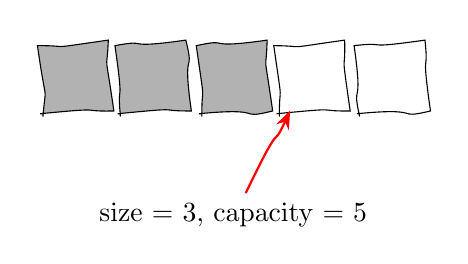
\begin{tikzpicture}[slot/.style={minimum size=0.9cm,rectangle}, data/.style={slot, fill=black!30}, >=Stealth, decoration=penciline]
        \matrix [nodes=draw] (table1)
        {
          \node[data, decorate] {}; &
          \node[data, decorate] {}; &
          \node[data, decorate] {}; & 
          \node[slot, decorate] (insert) {}; &
          \node[slot, decorate] {}; 
          \\ 
        };
        \node[below=of insert, xshift=-1cm] (start) {size = 3, capacity = 5};
        \draw[->,thick,red, decorate] (start) -- (insert);      
        \end{tikzpicture} 

        \column{0.65\textwidth}        
        We need to \textbf{resize the array}:

        \begin{enumerate}
            \item When size is too large, double the capacity
            \item When size is two small, half the capacity
        \end{enumerate}        
    \end{columns}

\end{frame}

\begin{frame}[fragile]
    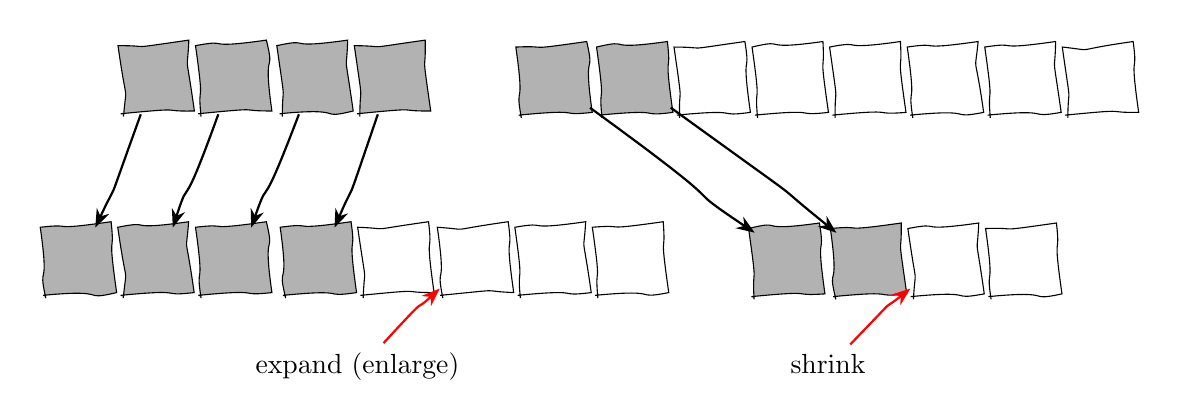
\begin{tikzpicture}[slot/.style={minimum size=0.9cm,rectangle}, data/.style={slot, fill=black!30}, >=Stealth, decoration=penciline]
    
    \matrix [nodes=draw](table2)
    {
      \node[data, decorate] (2n1) {}; &
      \node[data, decorate] (2n2) {}; &
      \node[data, decorate] (2n3) {}; & 
      \node[data, decorate] (2n4) {}; 
      \\ 
    };
    
    \matrix [nodes=draw, below=of table2, xshift=1cm](table3)
    {
      \node[data, decorate] (3n1) {}; &
      \node[data, decorate] (3n2) {}; &
      \node[data, decorate] (3n3) {}; & 
      \node[data, decorate] (3n4) {}; &
      \node[slot, decorate]  {}; &
      \node[slot, decorate] (insert2) {}; & 
      \node[slot, decorate] {}; & 
      \node[slot, decorate] {};   
      \\ 
    };
    
    \draw[->, thick, decorate] (2n1) -- (3n1);
    \draw[->, thick, decorate] (2n2) -- (3n2);
    \draw[->, thick, decorate] (2n3) -- (3n3);
    \draw[->, thick, decorate] (2n4) -- (3n4);
    
    \node[below=of insert2, xshift=-1.5cm, yshift=0.4cm] (start2) {\alert{expand} (enlarge)};
    \draw[->,thick,red,decorate] (start2) -- (insert2);

    
    \matrix [nodes=draw, right=of table2, xshift=-0.2cm](table4)
    {
      \node[data,decorate] (4n1) {}; &
      \node[data, decorate] (4n2) {}; &
      \node[slot, decorate] {}; & 
      \node[slot, decorate]  {}; &
      \node[slot, decorate] {}; &
      \node[slot, decorate] {}; & 
      \node[slot, decorate] {}; & 
      \node[slot, decorate] {}; 
      \\ 
    };

    \matrix [nodes=draw, below=of table4, xshift=1cm](table5)
    {
      \node[data, decorate] (5n1) {}; &
      \node[data, decorate] (5n2) {}; &
      \node[slot, decorate] (shrink) {}; & 
      \node[slot, decorate]  {};
      \\ 
    };
    \draw[->, thick,decorate] (4n1) -- (5n1);
    \draw[->, thick, decorate] (4n2) -- (5n2);

    \node[below=of shrink, xshift=-1.5cm, yshift=0.4cm] (start3) {\alert{shrink}};
    \draw[->,thick,red, decorate] (start3) -- (shrink);
    \end{tikzpicture} 
\end{frame}

\begin{frame}[fragile]
    \begin{minted}[baselinestretch=0.9,bgcolor=LightGray, fontsize=\small]{java}
private void resize(int capacity) {
    assert capacity >= n;
    a = Arrays.copyOf(a, capacity);
}

public void push(Item item) {
    if (n == a.length) resize(2 * a.length);
    a[n++] = item;
}

public Item pop() {
    if (isEmpty()) throw new NoSuchElementException();
    Item item = a[n-1];
    a[n-1] = null;
    n--;
    if (n > 0 && n == a.length / 4) resize(a.length / 2);
    return item;
}
    \end{minted}
\end{frame}

\begin{frame}
\section{\textcolor{darkmidnightblue}{Conclusion}}
    \begin{enumerate}
        \item Stack: LIFO
        \item Resizing (size vs. capacity)
        \item Iterator
    \end{enumerate}
\end{frame}

\begin{frame}
    \frametitle{Task}
    \begin{itemize}
        \item  Read \emph{``Application (2): arithmetic expression evaluation''} in Section 2.1.1.
        \item Exercise 2 in Chapter 2.
    \end{itemize}

\end{frame}

\end{document}